\section{Evaluering}
\begin{frame}{Testopsætning}
\begin{columns}
\begin{column}{0.6\textwidth}
Simulering af Hobrovej
\begin{itemize}
\item Trængsel baseret på GPS målinger og lokalt kendskab
\item Trafiksignaler baseret på 100 sekunders omløbstid
\item Fokus på nordgående retning af Hobrovej
\item Simulatorens brændstofs- udregninger (HBEFA-baseret)
\item Standardkørsel: Kører efter hastighedsgrænsen når muligt
\end{itemize}
\end{column}

\begin{column}{0.5\textwidth}
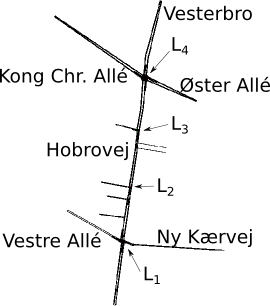
\includegraphics[width=1\textwidth]{../images/HobrovejNy.png}
\end{column}
\end{columns}
\end{frame}

\begin{frame}{Afstand - GPS målinger}
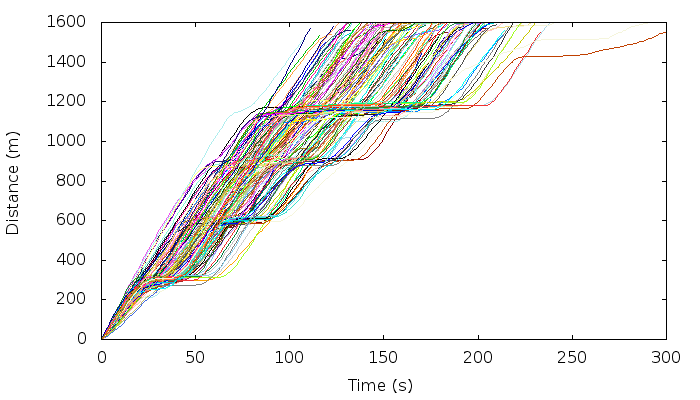
\includegraphics[width=1\textwidth]{../images/Real/RealDistance.png}

158 biler kørt i hverdage mellem 10:00 og 14:00
\end{frame}

\begin{frame}{Afstand - Simuleret standardkørsel}
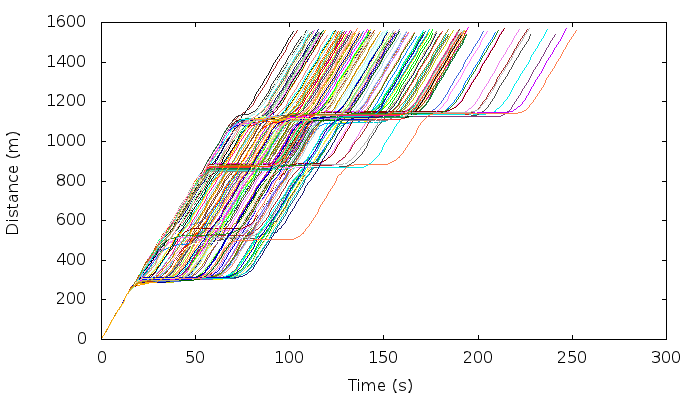
\includegraphics[width=1\textwidth]{../images/tp0c0_8/distanceUncontrolled0.png}

158 biler simuleret uden systemet
\end{frame}

\begin{frame}{Validering af simulatoren}

\begin{itemize}

\item SUMO med et trængselsniveau på 0.8 køretøjer per sekund
\item GPS data er samlet fra tidsrummet mellem kl 10 og 14 på hverdage
\end{itemize}

\centering
	\begin{tabular}{|l|c|c|c|c|}\hline
	 						&  \multicolumn{2}{c|}{SUMO} & \multicolumn{2}{c|}{GPS} \\\hline
	 						& Værdi & $\sigma$ & Værdi & $\sigma$ \\\hline
	gns. hastighed ($km/h$) 	& 37.45 & 7.86 	& 35.03 & 6.28 \\\hline
	gns. ventetid ($s$) & 66.90 & 33.97 & 70.35 & 33.07 \\\hline
	gns. antal stop 	& 1.91 	& 0.66 	& 1.80 	& 1.08 \\\hline
	\end{tabular}

\end{frame}

\begin{frame}{Afstand - 90 \% uden systemet}
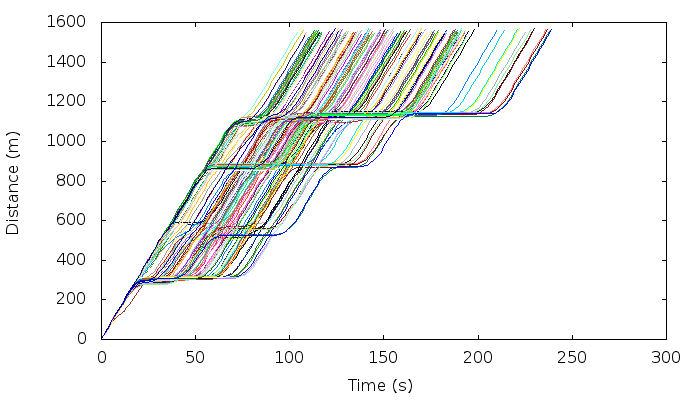
\includegraphics[width=1\textwidth]{../images/tp0c0_8/distanceUncontrolled10.png}

142 biler simuleret uden systemet
\end{frame}

\begin{frame}{Afstand - 10 \% med systemet}
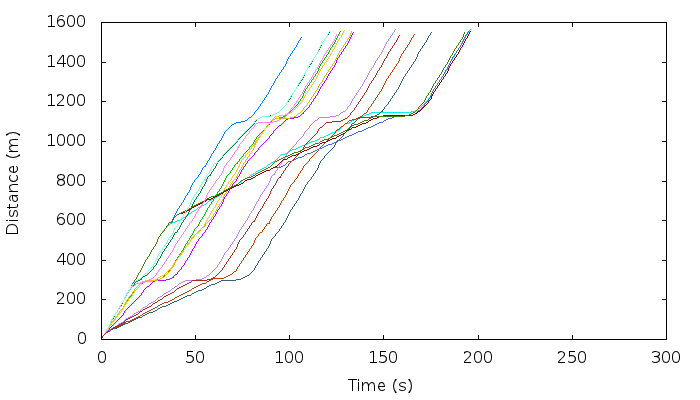
\includegraphics[width=1\textwidth]{../images/tp0c0_8/distanceControlled10.png}

16 biler simuleret med systemet
\end{frame}

\begin{frame}{Brændsstofforbrug - Sammenligning}
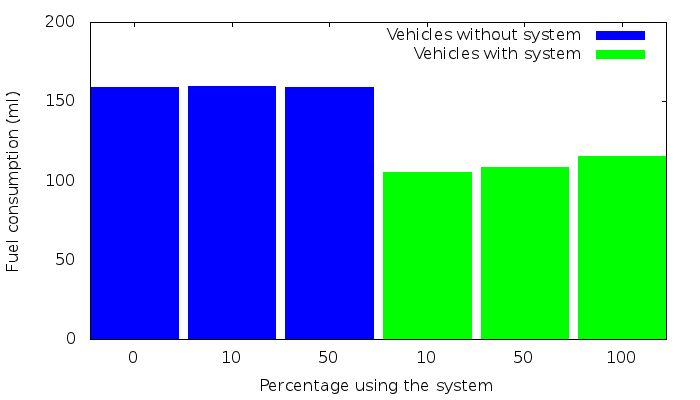
\includegraphics[width=1\textwidth]{../images/tp0c0_8/combinedFuel.png}
\end{frame}

\begin{frame}{Gennemsnitlig brændstofforbrug for alle biler}
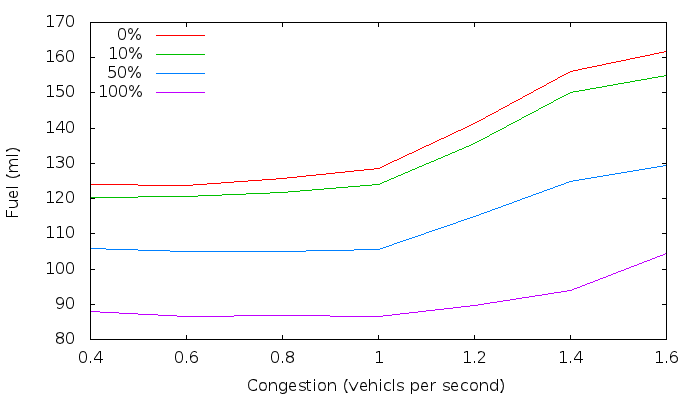
\includegraphics[width=1\textwidth]{../images/fuelCongestion.png}
\end{frame}

\begin{frame}{Gennemsnitlig rejsetid for alle biler}
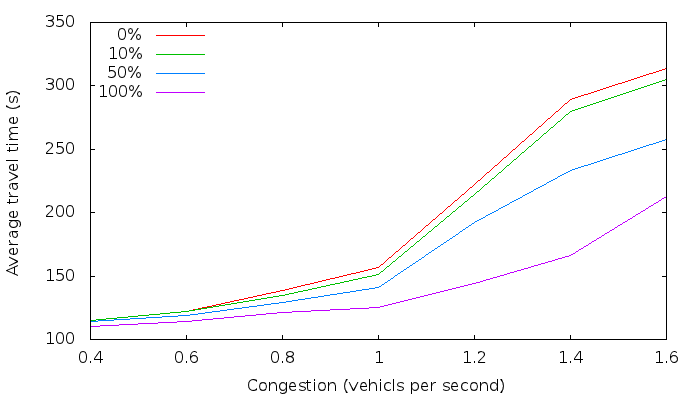
\includegraphics[width=1\textwidth]{../images/timeCongestion.png}
\end{frame}


\begin{frame}{Resultater}

\centering
\begin{tabular}{|l|l|cc|cc|}\hline
Procent brugere 			& Med/Uden & \multicolumn{2}{c|}{Brændstof} 	& \multicolumn{2}{c|}{Tid}\\
\tech					&\tech		& $ml$		& Forskel			&	$s$	& Forskel\\\hline
\multirow{1}{*}{0\%}	& Uden	&	125.8	&	0\%			&	139 & 0\%		\\\hline
\multirow{2}{*}{10\%}	& Med 		&	88.7	&	29.5\%		&	136 & 2.5\%		\\
						& Uden 	&	125.3	&	0.4\%		&	135 & 2.9\%		\\\hline
\multirow{2}{*}{50\%}	& Med		&	88.1	&	30.0\%		&	131 & 5.8\%		\\
						& Uden	&	121.8	&	3.2\%		&	127 & 8.6\%		\\\hline
\multirow{1}{*}{100\%}	& Med		&	86.8	&	31.0\%		&	121 & 12.9\%	\\\hline
\end{tabular}
Gennemsnitsværdier fra simuleringerne. Forskelen er beregnet i forhold til 0 \% brugere af \tech
\label{tb:TestResults:total}
\end{frame}